\documentclass[10pt,twocolumn,letterpaper]{article}
\usepackage[T1]{fontenc}
\usepackage[pagenumbers]{cvpr}
\usepackage{microtype}
\definecolor{cvprblue}{rgb}{0.16,0.30,0.50}
\usepackage[breaklinks,colorlinks,allcolors=cvprblue]{hyperref}
\graphicspath{{../results/figures/}}
\newcommand{\NyuAbsRel}{0.11455}
\newcommand{\NyuRMSE}{0.39889}
\newcommand{\NyuDelta}{0.89222}
\newcommand{\StereoMAE}{1.895}
\newcommand{\StereoCoverage}{75.69}
\newcommand{\TemporalGain}{18.23}
\newcommand{\EdgeRetention}{97.58}
\newcommand{\OriginalFPS}{2.77}
\newcommand{\EfficientFPS}{4.34}
\newcommand{\SpeedGain}{56.9}
\newcommand{\EfficientGain}{16.82}
\newcommand{\EfficientEdge}{97.64}

\newcommand{\MetricBaseAbs}{0.11455}
\newcommand{\MetricFinalAbs}{0.09564}
\newcommand{\MetricBaseRMSE}{0.39889}
\newcommand{\MetricFinalRMSE}{0.37080}
\newcommand{\MetricBaseDelta}{0.89222}
\newcommand{\MetricFinalDelta}{0.91374}
\newcommand{\MetricGain}{16.50}
\newcommand{\MetricCILow}{12.89}
\newcommand{\MetricCIHigh}{19.94}
\newcommand{\MetricReproduction}{0}
\newcommand{\MetricImproved}{431}
\newcommand{\MetricWorsened}{223}
\newcommand{\MetricBaseMS}{48.8}
\newcommand{\MetricFinalMS}{127.3}
\newcommand{\MetricMemory}{512}
\newcommand{\MetricReproductionSentence}{Reproduced and original baseline predictions differ by at most 0 m per pixel.}

\def\confName{CVPR}
\def\confYear{2027}
\title{Development-Calibrated Residual Refinement\\for Small-Model Monocular Metric Depth}
\author{Eugene\\HKUST (Guangzhou)\\AIAA 3201 Computer Vision Project}
\begin{document}
\maketitle
\begin{abstract}
We reproduce the revised course depth baselines and investigate lightweight adaptation of UniDepthV2 ViT-S. A scene-disjoint split of the 795 NYU development images reserves 577 images for fitting and 218 for selection. A controlled search compares global scale calibration, horizontal-flip averaging, and RGB-guided filtering. A small residual network learns spatial corrections to the strongest simple candidate while the pretrained depth network remains frozen. On all 654 NYU test images under the prescribed protocol, AbsRel changes from \MetricBaseAbs{} to \MetricFinalAbs{}, a \MetricGain\% reduction. RMSE changes from \MetricBaseRMSE{} to \MetricFinalRMSE{} m and $\delta_1$ from \MetricBaseDelta{} to \MetricFinalDelta{}. This is supervised development adaptation of an RGB-only reference. Shared-scale prediction and ground-truth error figures expose improvements and regressions. We also complete the 15-pair stereo exercise and required DA V2/VDA video comparison. The linked video contains only 70 genuine frames, leaving the 100-frame demo provisional. Code and results are available at \url{https://github.com/Lingxiaolingqc/MMDEVC/tree/feat/independent-performance-search/independent}.
\end{abstract}

\section{Introduction}
Consider a room surface whose true distance is 3 m. A predictor returning 2.4 m has 20\% proportional error. A multiplier of 1.25 would recover the correct value in this simplified example. In practice, errors vary with scene, distance, and boundaries, so one global multiplier can improve some regions while worsening others. This motivates testing more expressive corrections against measured depth labels.

The assignment combines calibrated stereo, quantitative monocular metric depth, qualitative relative-video comparison, and one improvement. We complete those requirements and select a metric refinement based on development evidence. The reference is unchanged UniDepthV2 ViT-S, one of the course's named recent research models. We preserve its checkpoint and inference preprocessing throughout the metric comparison.

Our contribution is a lightweight calibration/refinement stage fitted with the permitted NYU development data, together with independent evaluation, ablations, and failure analysis. The adaptation setting is stated alongside the original pretrained reference. We investigate how much error comes from global scale bias, whether reversible test-time averaging helps, and whether a small learned correction generalizes to scenes reserved from fitting.

An earlier flow-guided video experiment reduced a temporal-change proxy but had a small visible effect and supplied no metric-depth accuracy measurement. We therefore redirected the final improvement toward the course's quantitative task. Historical source and results remain available. The main accuracy evidence here uses NYU ground truth.

\section{Related Work}
Semi-global matching connects correspondence costs to calibrated stereo geometry~\cite{hirschmuller2008}. Middlebury includes fine structures and occlusions~\cite{scharstein2014}. KITTI~\cite{geiger2012} and TUM RGB-D~\cite{sturm2012} illustrate other evaluation settings, while this assignment uses the specified Middlebury and NYU data.

DPT introduced transformer-based dense prediction~\cite{ranftl2021}. Depth Anything and DA V2 provide strong relative-depth representations~\cite{yang2024da,yang2024dav2}. UniDepth/UniDepthV2 predict metric depth with camera-aware representations~\cite{piccinelli2024,piccinelli2025}, while Depth Pro is another metric reference named by the course~\cite{bochkovskii2025}. We choose UniDepthV2 ViT-S and compare its unchanged and refined outputs.

Video Depth Anything adds temporal modeling~\cite{chen2025}; optical flow such as RAFT~\cite{teed2020} supports correspondence-based propagation. The present metric adaptation instead operates on single RGB images, using NYU's Kinect-derived filled depth for evaluation~\cite{silberman2012}.

Guided filtering uses a local linear relationship to an image guide~\cite{he2010guided}. We test its luminance-guided form. Our learned refiner follows the general encoder-decoder and skip-connection structure of U-Net~\cite{ronneberger2015unet}, using independently trained parameters and a bounded multiplicative correction.

\section{Data and Evaluation}
\subsection{Scene-Disjoint NYU Development}
The labeled MAT and official split provide 795 development and 654 test images. MATLAB indices are converted to zero-based IDs. RGB is read as \texttt{images[i].transpose(2,1,0)} and filled metric depth as \texttt{depths[i].T}. Mirror transport, the whole-file hash, field shapes, and a matching prefix from the university download are recorded.

We divide development images by complete scene names. Sorting scenes and shuffling with seed 320112 reserves 62 scenes for validation, yielding 577 fitting images and 218 validation images. The fitting and validation scenes are disjoint, and no official test IDs enter development. Calibration and gradients use fitting labels. Candidate and checkpoint selection use validation scores.

The earlier 654-image baseline and some of its failures had already been inspected during the project. This history is disclosed. The new search uses development measurements, and the final configuration and checkpoint digest are committed before the new test run.

\subsection{Course Protocol}
Predictions are evaluated at $480\times640$ with crop $[45:471,41:601]$. GT must be finite, strictly above 0.001 m and below 10 m. Predictions are clipped to $[0.001,10]$ m. Non-finite model outputs fail evaluation. All candidates share this support and arithmetic.

AbsRel averages $|p-g|/g$ for prediction $p$ and truth $g$. RMSE is the square root of mean squared error. $\delta_1$ counts ratios $\max(p/g,g/p)<1.25$. Metrics are computed per image and averaged equally. Development-fitted corrections remain fixed during testing. There is no test-label-based scale fitting.

AbsRel is the selection metric, with RMSE and $\delta_1$ reported alongside it. Paired per-image records reveal gains and regressions. A 5,000-replicate scene-cluster bootstrap resamples whole test scenes to estimate uncertainty in relative AbsRel reduction.

\subsection{Stereo and Video Inputs}
Stereo uses all 15 Middlebury quarter-resolution pairs, their calibration, and \texttt{disp0GT.pfm}. The official ZIP names the folder \texttt{trainingQ}, corresponding to the brief's \texttt{trainQ} shorthand.

The linked rollercoaster source decodes to 70 frames at $960\times540$, 24 FPS, with SHA-256 beginning \texttt{7268cbec}. Both relative models process all genuine frames at $640\times360$ output. DA V2-Small uses input size 518. VDA-Small uses offline FP16 inference and main input size 392 after the allowed memory reduction. Required preprocessing remains model-specific.

Each relative model uses a fixed whole-clip 2nd/98th percentile display range and the same palette. Equal colors across models have no common metric-distance meaning. No true depth or camera poses are supplied for this video. Its comparison remains qualitative. A longer official copy or clarification is needed for literal 100-frame compliance.

\section{Metric Refinement}
\begin{figure*}[t]
\centering
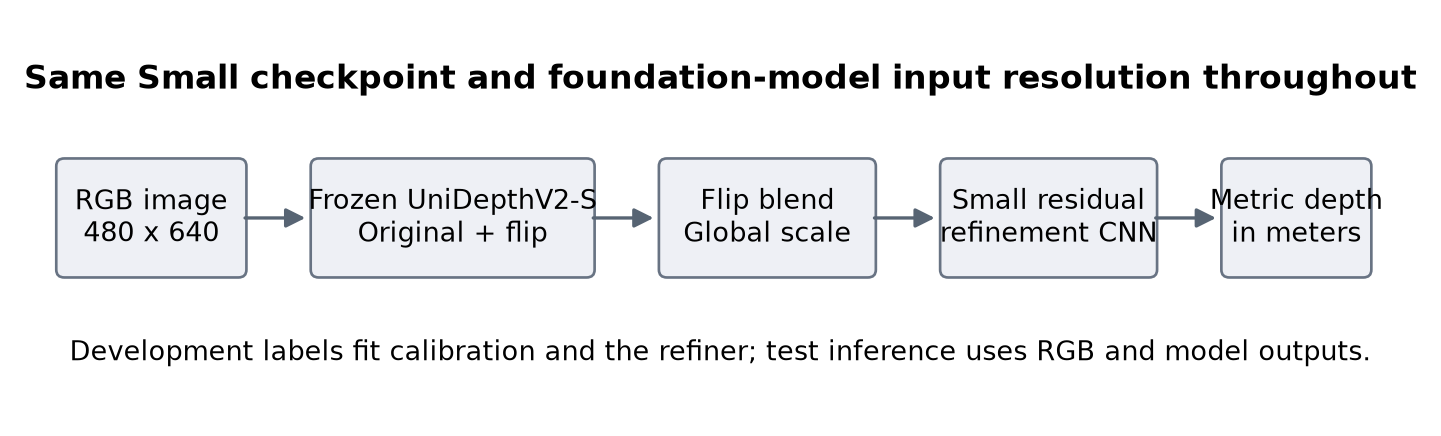
\includegraphics[width=\textwidth]{metric-pipeline.png}
\caption{The final metric improvement. Frozen UniDepthV2-S runs on original and flipped RGB at the same foundation input resolution. A development-fitted blend and scale produce a base map. A small RGB-guided network adds bounded spatial log corrections. Test inference uses RGB and model outputs.}
\label{fig:pipeline}
\end{figure*}

\subsection{Frozen Foundation and Simple Candidates}
We use the official \texttt{unidepth-v2-vits14} checkpoint and RGB-only \texttt{infer(rgb)} with its default FP16 behavior. The official implementation rounds $480\times640$ input to an internal $490\times644$. Checkpoint, normalization, and resolution settings remain fixed.

Let $p=F(I)$ be the original metric prediction. A second pass on horizontally flipped RGB is flipped back into original coordinates to produce $p_f$. We form
\begin{equation}
b=s\bigl((1-w)p+w p_f\bigr).
\end{equation}
The pretrained parameters belong to $F$. We cache both depth outputs and the original model's confidence map, treating confidence as a feature without assuming calibrated probabilities.

Flip weights are $0,0.25,0.5,0.75,1$. Each blend is evaluated with scale 1 and a development-fitted global scale. Fitting samples the prescribed crop on a fixed eight-pixel grid. The sampled unclipped AbsRel objective gives a weighted median of $g/p$, with weights proportional to $p/(Ng)$ where $N$ is the valid sample count in that fitting image.

For original and equal-flip calibrated predictions we also test guided filtering with radii 2, 4, 8 and regularization $10^{-4},10^{-3},10^{-2}$. The resulting 28 candidates are scored on all 218 reserved images with the exact full-resolution protocol.

The strongest simple candidate uses $w=0.25$ and $s=0.9413383$. Its validation AbsRel is 0.10821, compared with 0.12069 for the unchanged reference. Global scaling supplies most of this gain. Guided filtering and stronger averaging provide no better selection score.

\subsection{Small Learned Correction}
Features contain RGB, log original depth, log restored-flip depth, log base depth, transformed confidence, and normalized horizontal/vertical coordinates. RGB contributes appearance and boundaries, the frozen maps supply geometry, and coordinates permit learning domain-specific spatial regularities. GT never enters the inference features.

The refiner operates at $240\times320$. Encoder widths are 16, 32, 64, 96 with three average-pooling stages. Bilinear decoder upsampling concatenates encoder features through skip connections. Blocks use group normalization and GELU. There are 388,001 parameters.

The network predicts a bounded log residual,
\begin{equation}
r=0.5\tanh R_\theta(x), \qquad
\widehat p=b\exp(\operatorname{resize}(r)).
\end{equation}
The correction factor lies between approximately 0.607 and 1.649. A zero-initialized output layer makes the initial refiner reproduce the simple base exactly, which is checked numerically. The full-resolution base carries detail through the multiplicative output path.

\subsection{Fitting and Selection}
AdamW trains only the refiner, with learning rate $3\times10^{-4}$, weight decay 0.001, batch size 8, gradient clipping at 1, and FP16 autocast. A cosine schedule targets 80 epochs with minimum rate $10^{-5}$. Fitting minimizes equal-image AbsRel on the downsampled valid crop. Selection always uses the exact full-resolution course evaluation.

Validation is measured at epoch 1 and every two epochs. A 20-epoch patience rule after a minimum of 24 epochs stops training at epoch 50 and selects epoch 30. Validation AbsRel is 0.10275, a 14.86\% reduction from its unchanged reference. The checkpoint is saved as safetensors with its digest.

This is supervised NYU development adaptation. Its scope differs from a fully zero-shot benchmark. The comparison measures improvement over the named course reference under the permitted adaptation procedure.

\section{Results}
\begin{table}[t]
\centering
\caption{All 654 NYU test images under one course protocol. Calibration/refinement use development supervision.}
\resizebox{\columnwidth}{!}{\begin{tabular}{lrrr}
\toprule Method & AbsRel & RMSE (m) & $\delta_1$\\
\midrule
Unchanged UniDepthV2-S & 0.11455 & 0.39889 & 0.89222\\
Global scale only & 0.10151 & 0.39484 & 0.89714\\
Flip averaging only & 0.11427 & 0.39640 & 0.89432\\
Selected flip + scale & 0.10109 & 0.39251 & 0.89939\\
Residual refinement & 0.09564 & 0.37080 & 0.91374\\
\bottomrule
\end{tabular}
}
\label{tab:metric}
\end{table}

\subsection{Metric Accuracy and Ablations}
The final method obtains AbsRel \MetricFinalAbs{}, RMSE \MetricFinalRMSE{} m, and $\delta_1=\MetricFinalDelta$. Table~\ref{tab:metric} gives the paired reference and ablations. AbsRel falls by \MetricGain\%. \MetricReproductionSentence{}

The scene-cluster bootstrap 95\% interval for relative AbsRel reduction is \MetricCILow\% to \MetricCIHigh\%. Of 654 images, \MetricImproved{} improve and \MetricWorsened{} worsen. This interval describes sampling variation over these scenes, with additional uncertainty from method selection and future conditions.

\begin{figure*}[t]
\centering
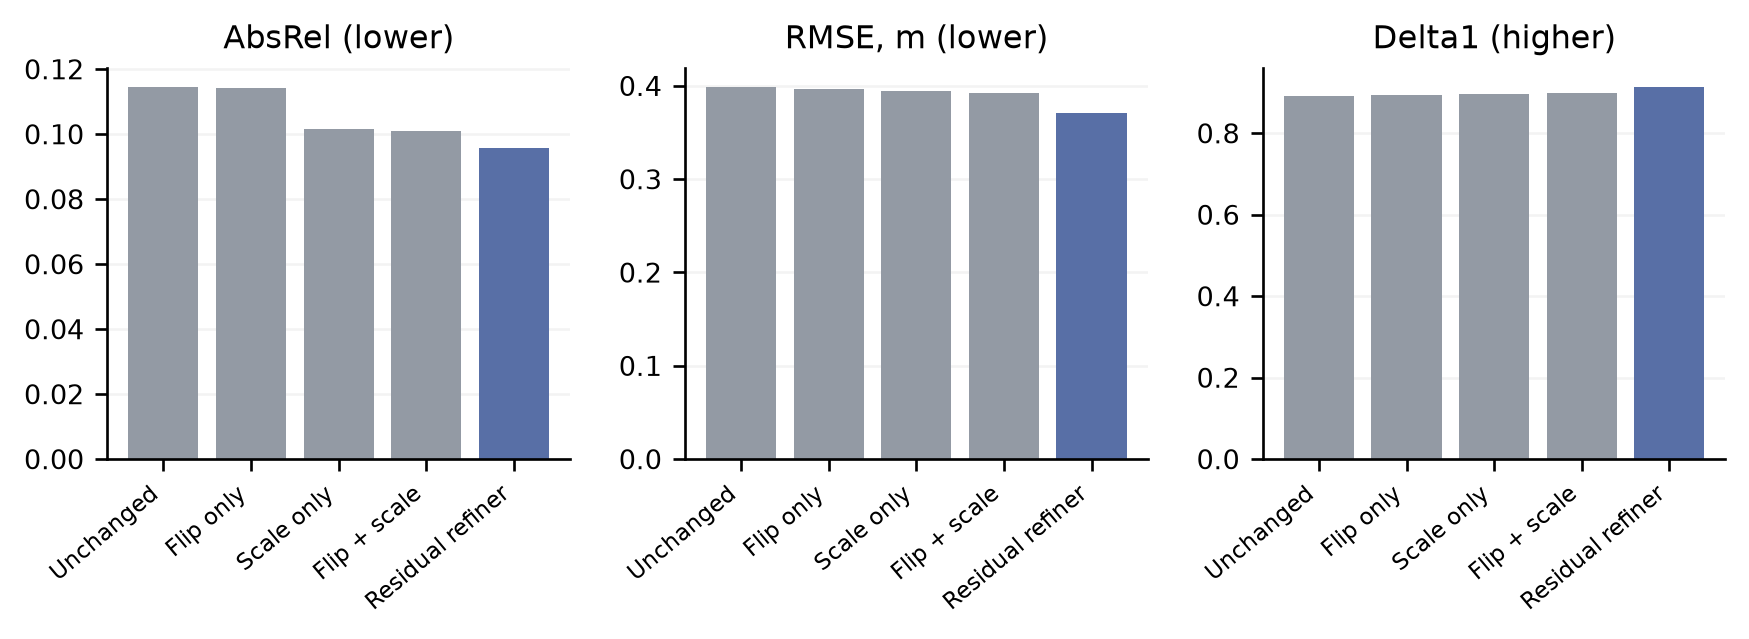
\includegraphics[width=\textwidth]{metric-ablation.png}
\caption{Ablations use identical test IDs, crop, support, output size, and aggregation. Flip averaging, global calibration, and the residual network have separately measured contributions. Foundation checkpoint and input resolution are fixed.}
\label{fig:ablation}
\end{figure*}

Flip-only averaging measures sensitivity to a reversible transformation. Global calibration measures scale bias. The simple combination tests their interaction, and the residual network measures spatial adaptation beyond that base. The development search shows that added computation can worsen accuracy. Equal-flip averaging raises validation AbsRel before scaling, and guided-filter candidates fail to beat the selected blend.

The refiner's fitting loss can decrease while validation error rises. An earlier checkpoint therefore wins over the final training epoch. We retain the complete curve and every validation evaluation. The 62 held-out scenes reduce direct room memorization, while leaving uncertainty about unfamiliar domains.

\begin{figure*}[t]
\centering
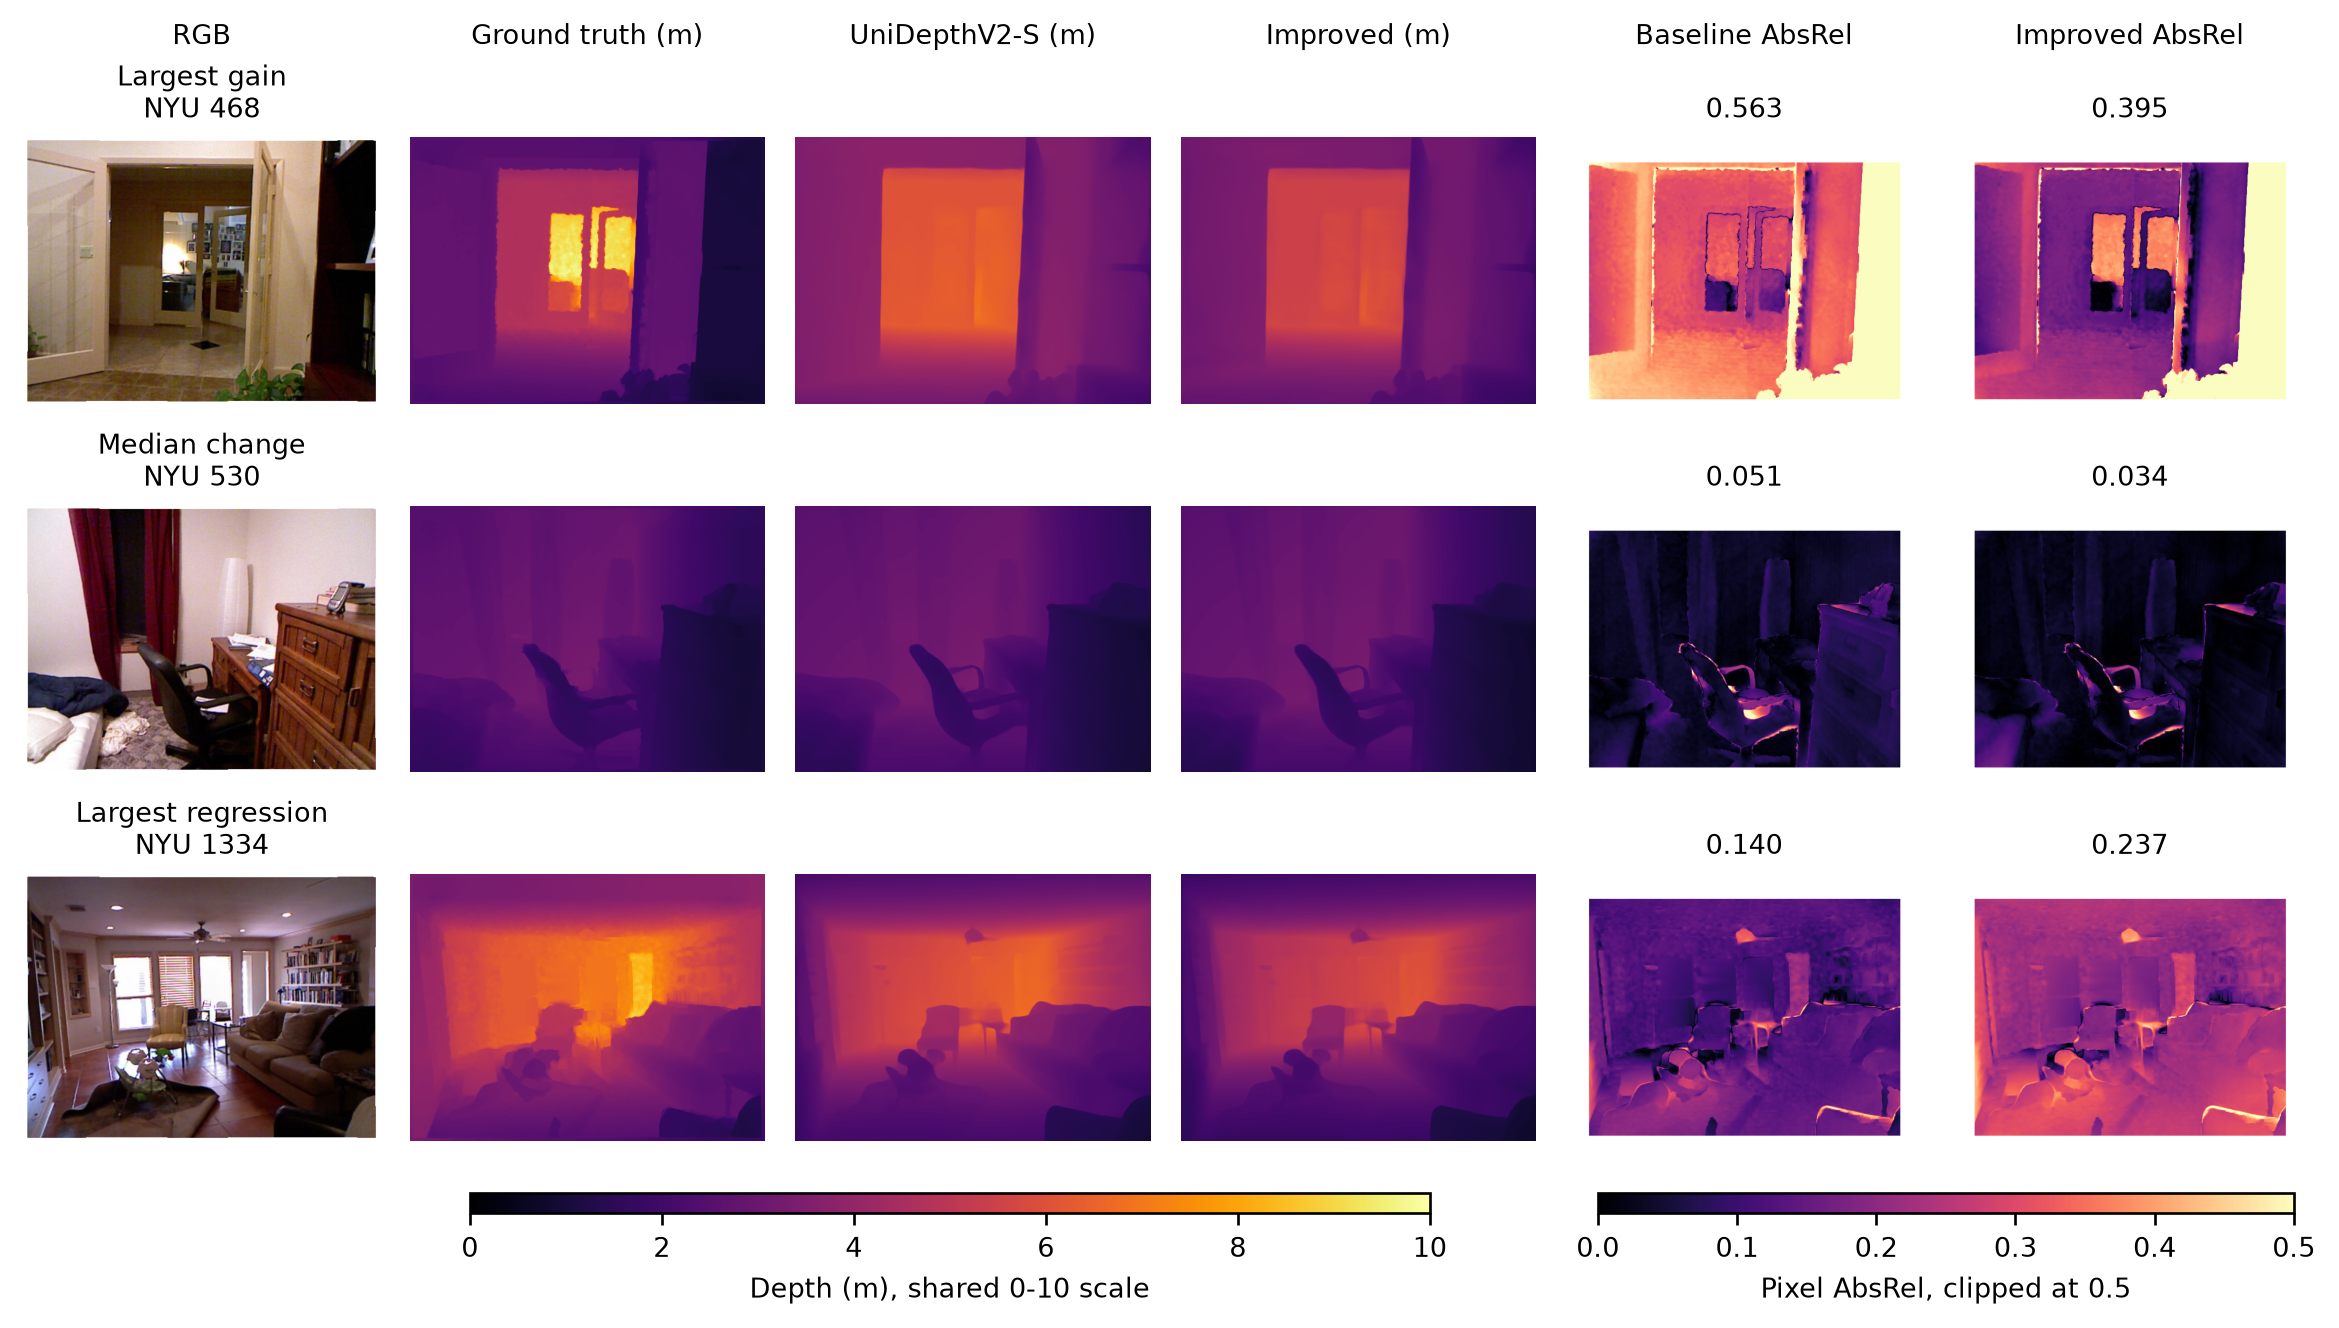
\includegraphics[width=\textwidth]{metric-comparison.png}
\caption{Ground-truth comparisons with shared 0--10 m depth colors and shared 0--0.5 pixel AbsRel colors. Rows are selected by largest per-image gain, median change, and largest regression. Error maps use only the course evaluation crop.}
\label{fig:comparison}
\end{figure*}

\subsection{Visual Evidence and Failures}
Figure~\ref{fig:comparison} compares predictions directly with GT. Common depth and error scales prevent display normalization from imitating an accuracy gain. The regression row makes visible where adaptation damages an individual example.

Filled NYU depth contains Kinect measurements and inpainting, with ambiguity near missing measurements and boundaries. The original baseline's three largest-AbsRel images, 468, 87, and 516, show interior scale disagreement, cluttered layers, and thin chair geometry near a bright window. Their selection predates the refinement search.

\begin{figure*}[t]
\centering
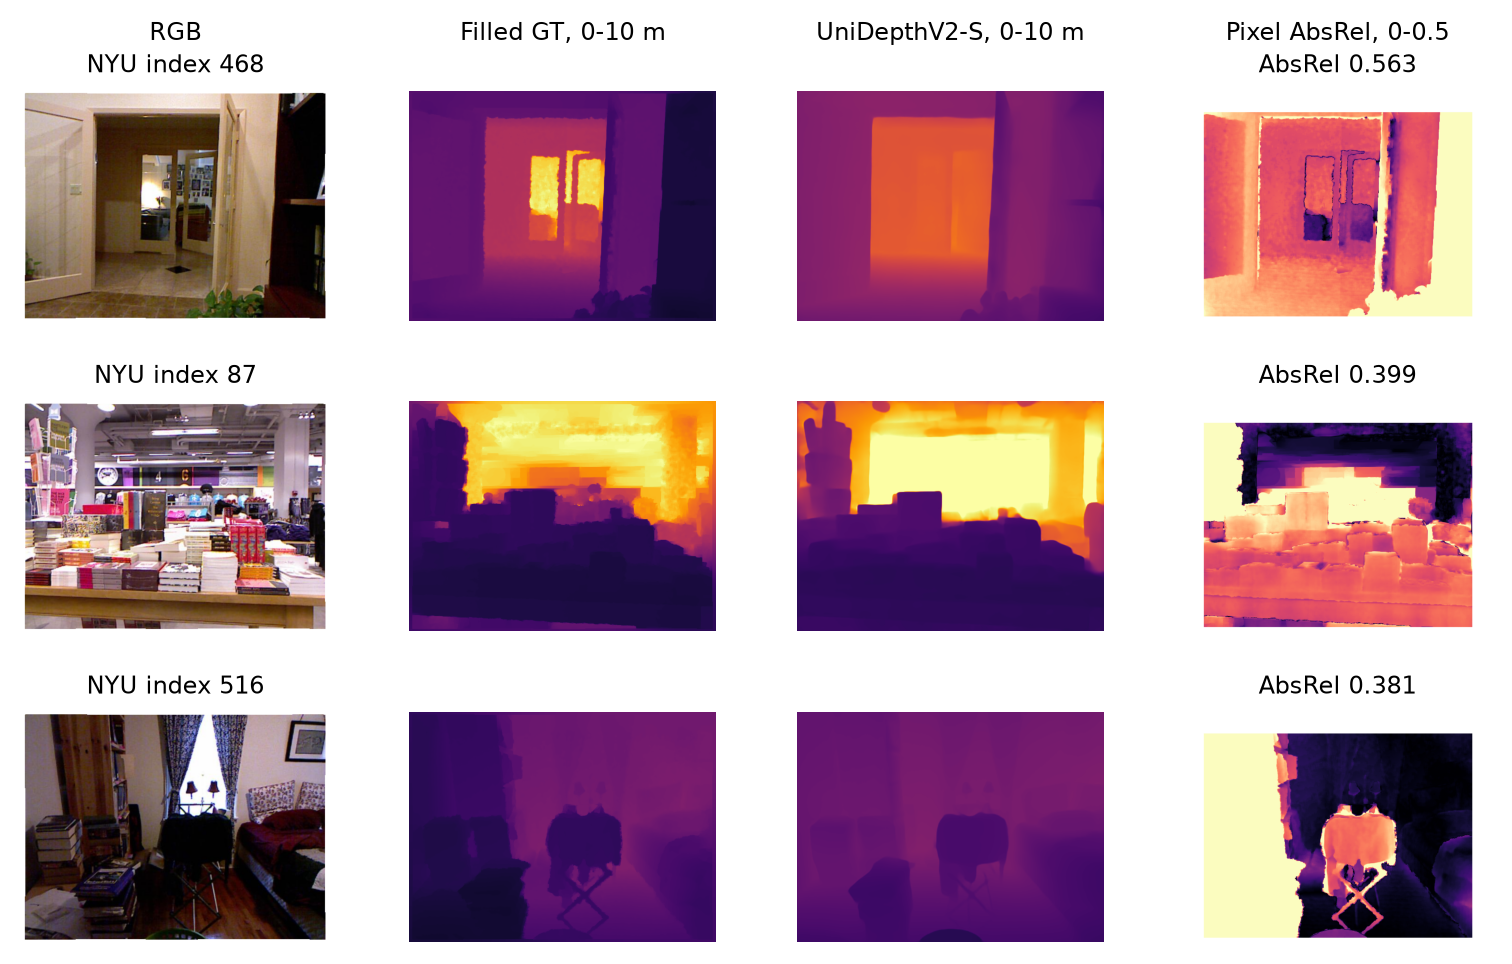
\includegraphics[width=.93\textwidth]{nyu-failures.png}
\caption{The baseline's three highest-AbsRel NYU images, chosen automatically in the earlier baseline run. GT and prediction use shared 0--10 m colors. These actual difficult cases motivate scale/boundary analysis and remain disclosed alongside new gain/regression examples.}
\label{fig:failures}
\end{figure*}

The residual model may encode development-domain spatial priors or transfer appearance texture into depth. Reflective surfaces, unusual layouts, and ambiguous filled labels can cause failure. Additional RGB-D domains would be needed to establish broader robustness.

\subsection{Mandatory Stereo Exercise}
OpenCV fixed-point disparity $r$ is converted to pixels as $d=r/16$. Focal length $f$, baseline $B$ in millimeters, and calibration offset give
\begin{equation}
z=\frac{fB}{d+\mathrm{doffs}}\frac{1}{1000}.
\end{equation}
For $r=160$, $f=1000$, $B=100$, and $\mathrm{doffs}=2$, disparity is 10 pixels and depth is 8.333 m. We use quarter-resolution calibration and exclude invalid disparities.

SGBM uses block size 5, $P_1=200$, $P_2=800$, uniqueness 10, speckle window 100, and 3WAY mode. Search range is the calibration range rounded up to a multiple of 16. All 15 pairs yield mean pair MAE \StereoMAE{} px and mean coverage \StereoCoverage\%. MAE uses the intersection of positive finite prediction and GT support; coverage uses all valid GT as denominator.

\begin{figure*}[t]
\centering
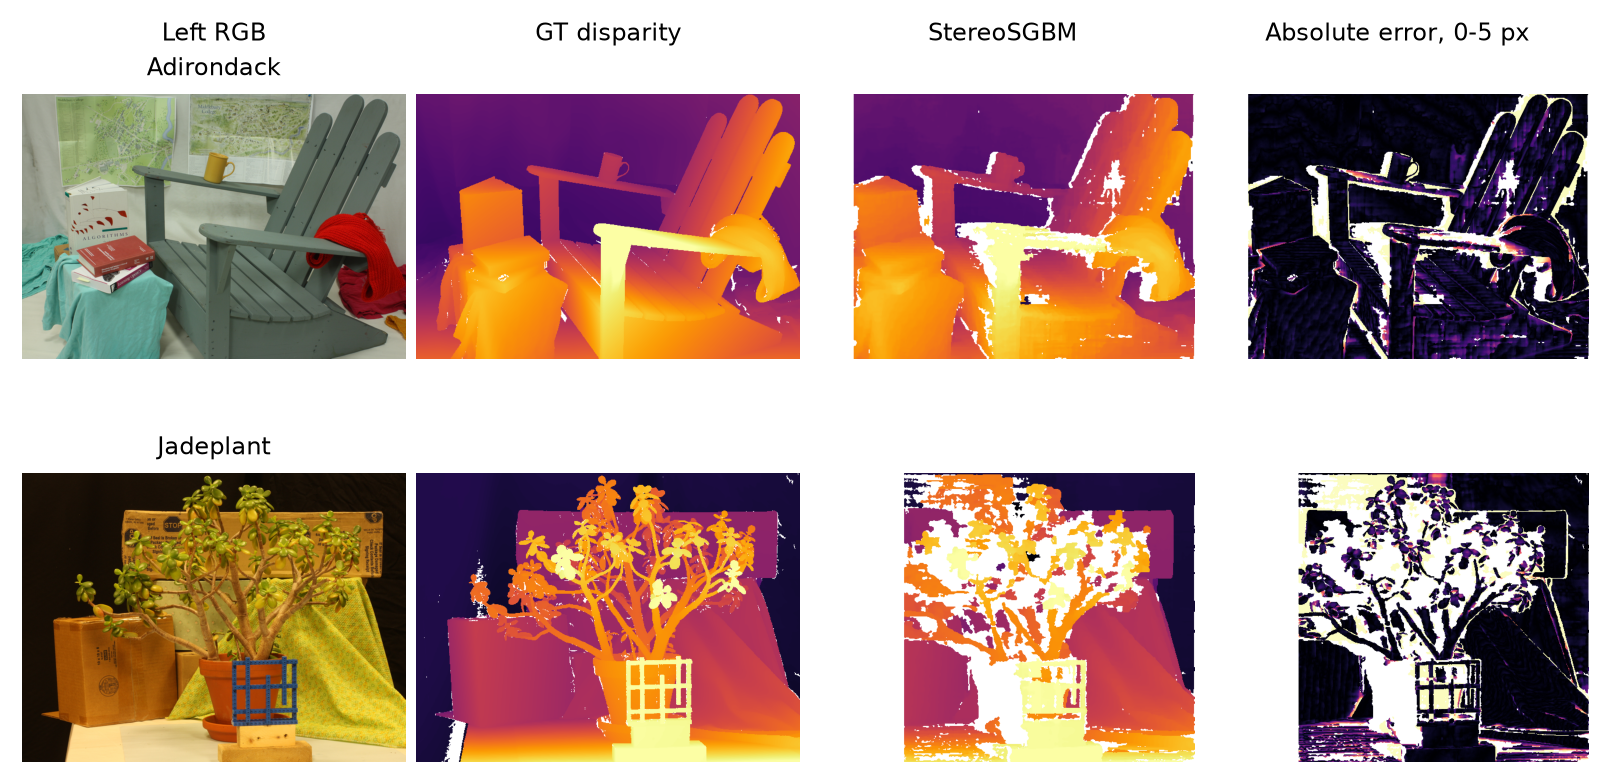
\includegraphics[width=.9\textwidth]{stereo-comparison.png}
\caption{Independent stereo on Adirondack and Jadeplant. Disparity ranges are shared within each pair. Invalid predictions are masked and display error is capped at 5 px. Thin leaves and occlusion remain difficult, with coverage reported alongside error.}
\label{fig:stereo}
\end{figure*}

\subsection{Required Relative-Video Comparison}
Figure~\ref{fig:video} shows genuine chronological frames 0, 35, and 69. DA V2 and VDA recover large track structure, with differences at thin supports and moving boundaries. Fixed per-model ranges support temporal inspection. The fourth panel preserves the earlier fusion experiment for continuity with saved videos.

Its mean absolute prediction change was only 0.22\% of the unchanged display range. This explains the subtle visual effect. Its temporal-proxy gain concerns stability, while the final metric improvement here is evaluated against NYU GT.

\begin{figure*}[t]
\centering
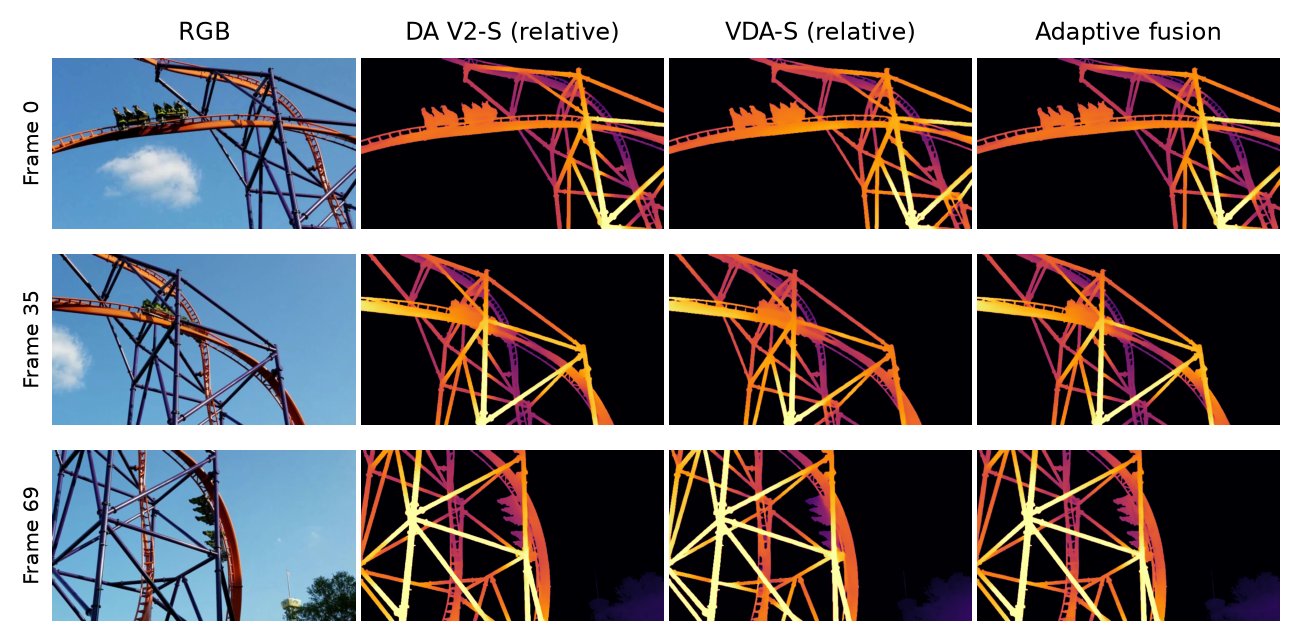
\includegraphics[width=\textwidth]{video-comparison.png}
\caption{Required RGB/DA V2/VDA comparison. The fourth column preserves earlier temporal fusion. DA V2 and fusion share one fixed range; VDA has its own. All outputs preserve genuine source frames and original FPS.}
\label{fig:video}
\end{figure*}

\subsection{Runtime and Application}
Runs use an RTX 4070 Laptop GPU with 8,188 MiB VRAM, Python 3.12.6, PyTorch 2.8.0/CUDA 12.8, and OpenCV 4.11.0.86. Median fresh reference inference is \MetricBaseMS{} ms/image and improved inference \MetricFinalMS{} ms/image. Improved time includes both foundation passes, feature preparation, residual inference, and resize, with file I/O, metrics, and compression excluded. Peak allocated memory is \MetricMemory{} MiB.

VDA input 518 took 73.49 s for 70 frames and reported 8,014 MiB allocated/11,858 MiB reserved. Permitted input 392 took 6.94 s with 3,072/4,194 MiB. Logical Windows CUDA counters do not directly establish physical residency. Both settings are retained, with 392 used for the main reference.

The metric application uses background blur with a shared 3 m focus threshold, 0.4 m transition, and Gaussian blur for baseline and improved depth. The focus threshold is chosen manually to expose near/far regions in the displayed example. The associated figure demonstrates how the metric correction affects an application. The original recorded video application is also retained.

\begin{figure*}[t]
\centering
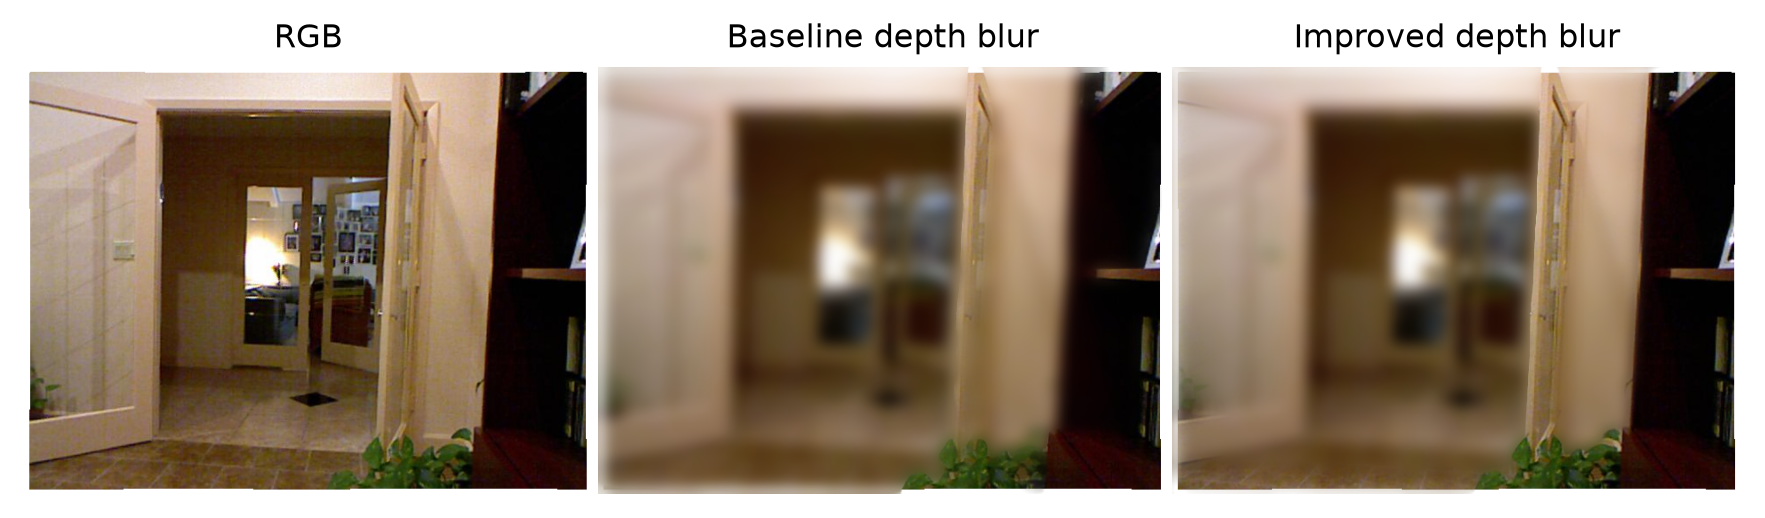
\includegraphics[width=\textwidth]{metric-application.png}
\caption{Same RGB image and blur settings using baseline and refined metric depth. Focus remains sharp below approximately 3 m with a 0.4 m transition. The example is the largest-AbsRel-gain image from the declared rule.}
\label{fig:application}
\end{figure*}

\section{Reproducibility and Limitations}
Source, tests, settings, and measured summaries live in an independent directory/feature branch. Foundation weights and datasets remain external. The small refiner is included as safetensors. Input hashes, split IDs, settings, training curves, paired CSV rows, and raw predictions support reproduction.

Early runs predated automatic source-snapshot hashing; their missing hashes are not reconstructed. New records capture source/Git/config identities. The metric configuration and weight digest were committed before final testing. Tests cover units, crops, equal-image aggregation, scale fitting, blending, constant-map filtering, identity refinement, and CLI integration.

The result concerns adaptation on one indoor dataset. Development supervision and extra inference passes change the operating setting relative to the original pretrained reference. The bootstrap interval omits selection uncertainty. Cross-camera and outdoor performance remain unmeasured. We retain per-image regressions and the limitations of filled GT.

The 70-frame source leaves the literal 100-frame requirement unresolved. Packaging requires explicit provisional mode and includes a warning. The draft author line also needs group confirmation. Official architectures, checkpoints, and template remain attributed. Worked examples and learning notes accompany the implementation.

\section{Conclusion}
The selected development-calibrated residual refinement reduces NYU AbsRel by \MetricGain\% against the course's UniDepthV2-S reference under the same test protocol. Simple candidates identify global bias, while the small RGB-guided network adds spatial correction. Paired GT error maps expose gains and regressions. Required stereo and video exercises are reproduced with explicit units, masks, display ranges, and source limitations.

\clearpage
\twocolumn
{\small
\bibliographystyle{ieeenat_fullname}
\bibliography{references}
}
\end{document}
